\documentclass[a4paper]{jsarticle}

%======================================================================
%		論文のタイトル,著者,日付
%======================================================================

\title{\Huge データマイニング工学\\\huge 第3回レポート\vspace{120mm}}
\author{\Large 濱崎 直紀\\\large (学籍番号:28G19096)\vspace{25mm}}
\date{令和2年2月3日}

%======================================================================
%		マクロの読み込みとコマンドの定義
%======================================================================

\usepackage{graphicx}       % eps fileを張り付けるのに必要
% \usepackage[dvipdfmx]{graphicx}     % png等の画像を貼りつけるのに必要
\usepackage{bm}     % 太字を書くのに必要
\usepackage{here}       % その場所に画像を入れるのに必要
\usepackage{comment}        % コメントを挟むのに必要
\usepackage{listings}      % ソースコードを表示するのに必要
\usepackage{jlisting}       % ソースコード内に日本語のコメントアウトがある場合必要(TEX Liveの場合,別途ダウンロードが必要)
\usepackage{caption}

%======================================================================
%		本文
%======================================================================

\begin{document}

\begin{titlepage}
\maketitle
\thispagestyle{empty}
\end{titlepage}

\section*{問題1}
問題3で示す.
\section*{課題2}
今後,エネルギーの効率的な利用に情報通信技術はますます欠かせないものとなりますが,情報通信技術を活かし,ピーク電力抑制や省エネなど電力の効率的な利用を推進していくためには,どのような施策を実施すればよいか,ご自身の考えをまとめてください. 

\subsection*{(回答)}
私が考えた施策は,使用されていない間,機能を停止することで消費電力を抑制するというものである.
より具体的には,ユーザーが利用しているかどうかを把握するシステムさえあれば,ユーザーが使用していない間は機能を停止させることで,大幅な電力の削減が見込めるというものである.
しかし実際には,使用時間と通信機能のオンオフを完全に同期させることは難しいと思う.
そのような問題に対して,今後機械学習などを活用して,どの時間にどれだけ通信に需要があるのかということを学習させ,AIによって自動的にオンオフ,また,完全に停止させなくとも,どれだけ抑制させるかということを機械に制御させるということが可能になれば,電力の削減に非常に大きく貢献すると思った.

\section*{問題3}
$\hat{c}_1$, $\hat{c}_{\rm rand}$, $\hat{c}_{\rm min}$の分布をヒストグラムで表すと,それぞれ以下の図のようになる.
\begin{figure}[H]
    \begin{center}
        \includegraphics[width=100mm]{./figures/section_3/c_1.eps}
        \captionsetup{labelformat=empty,labelsep=none}
        \caption{$\hat{c}_1$}
    \end{center}
\end{figure}
\begin{figure}[H]
    \begin{center}
        \includegraphics[width=100mm]{./figures/section_3/c_rand.eps}
        \captionsetup{labelformat=empty,labelsep=none}
        \caption{$\hat{c}_{\rm rand}$}
    \end{center}
\end{figure}
\begin{figure}[H]
    \begin{center}
        \includegraphics[width=100mm]{./figures/section_3/c_min.eps}
        \captionsetup{labelformat=empty,labelsep=none}
        \caption{$\hat{c}_{\rm min}$}
    \end{center}
\end{figure}
\section*{問題4}
\begin{enumerate}
    \renewcommand{\labelenumi}{\Alph{enumi}.}
    \item (B)で示す.
    \item
    $\hat{c}_1$, $\hat{c}_{\rm rand}$, $\hat{c}_{\rm min}$の3種類のコインにおいて,$\bm{{\rm P}}\{|\hat{c}-\bm{{\rm E}}c|>\varepsilon\}$を近似し,$\varepsilon$の関数としてそのグラフを描くと,以下の図のようになる.
    尚,同じプロットにおいて,Hoeffdingの上界($2e^{-2\varepsilon^2n}$)をオレンジの線で表している.
    \begin{figure}[H]
        \begin{center}
            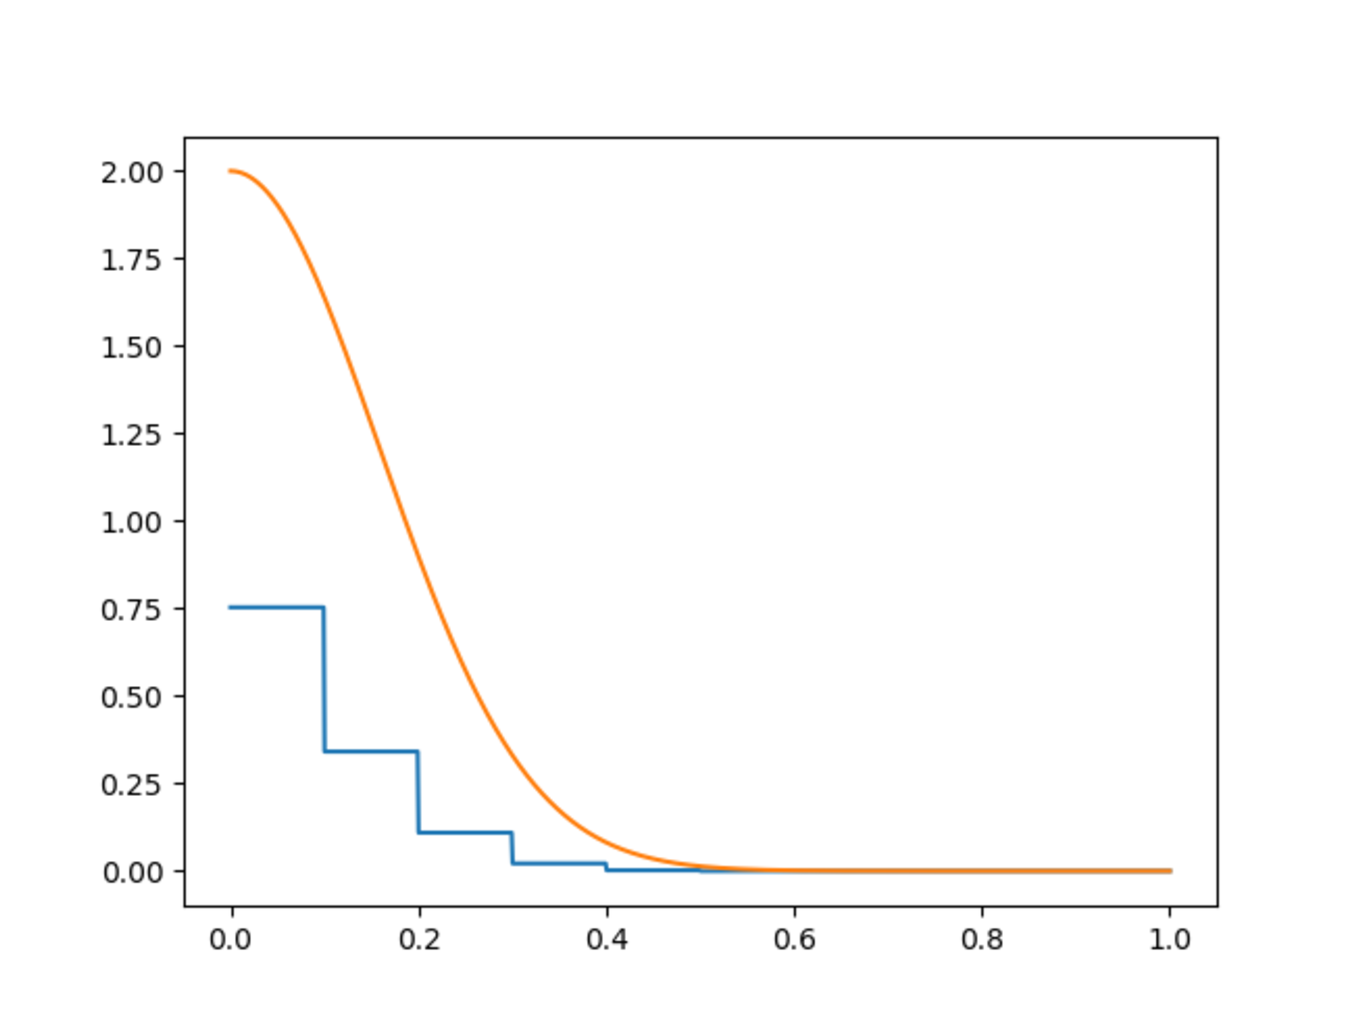
\includegraphics[width=100mm]{./figures/section_4/Hoeffding_c1.eps}
            \captionsetup{labelformat=empty,labelsep=none}
            \caption{$\hat{c}_1$}
        \end{center}
    \end{figure}
    \begin{figure}[H]
        \begin{center}
            \includegraphics[width=100mm]{./figures/section_4/Hoeffding_crand.eps}
            \captionsetup{labelformat=empty,labelsep=none}
            \caption{$\hat{c}_{\rm rand}$}
        \end{center}
    \end{figure}
    \begin{figure}[H]
        \begin{center}
            \includegraphics[width=100mm]{./figures/section_4/Hoeffding_cmin.eps}
            \captionsetup{labelformat=empty,labelsep=none}
            \caption{$\hat{c}_{\rm min}$}
        \end{center}
    \end{figure}
    \item
    $c_1$と$c_{\rm rand}$はHoeffdingの不等式に従うが,$c_{\rm min}$は従わない.
    これは,$c_{\rm min}$が1000枚のコインの中の任意のコインではなく,表の数が最も少なかった特定のコインであるからである.
\end{enumerate}
\section*{問題5}
標本数$n$(コインを投げる回数)を500としたときの$\hat{c}_{\rm min}$の分布のヒストグラムは以下のようになる.
\begin{figure}[H]
    \begin{center}
        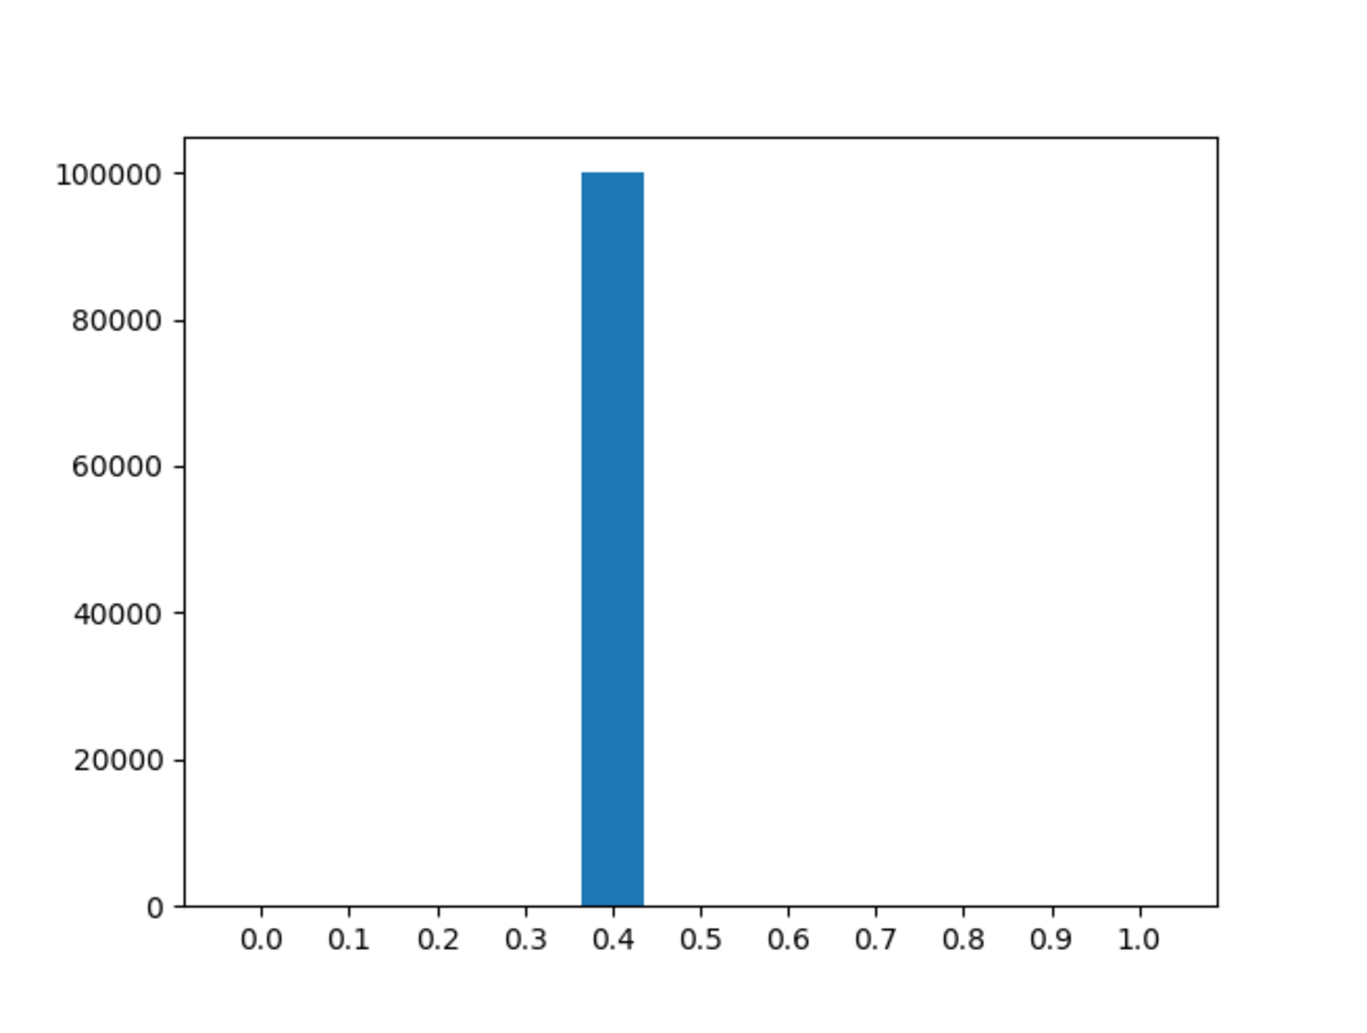
\includegraphics[width=100mm]{./figures/section_5/c_min_500.eps}
        \captionsetup{labelformat=empty,labelsep=none}
        \caption{$\hat{c}_{\rm min}$($n=500$)}
    \end{center}
\end{figure}

標本数が10である問題3の$\hat{c}_{\rm min}$では,分布が$\hat{c}=0.0,\ 0.1$(コインが表である割合)に集まっているのに対して,標本数が500のときは分布が$\hat{c}=0.4$に集まっている.
標本数が10のように少ない場合は,1000枚のコインの中に期待値$\hat{c}=0.5$から大きく外れた$\hat{c}$の非常に小さいコインが紛れている可能性は非常に高い.
しかし,標本数が500のように多い場合は,確率が収束し,$\hat{c}$が最も小さいコインでも期待値から大きく外れず,分布が$\hat{c}=0.4$辺りに集まっていると考えられる.

%======================================================================
%		付録
%======================================================================

\clearpage
\appendix
\pagestyle{empty}
% ソースコードの表示に関する設定
\lstset{
    basicstyle={\ttfamily},
    identifierstyle={\small},
    commentstyle={\smallitshape},
    keywordstyle={\small\bfseries},
    ndkeywordstyle={\small},
    stringstyle={\small\ttfamily},
    frame={tb},
    breaklines=true,
    columns=[l]{fullflexible},
    numbers=left,
    xrightmargin=0zw,
    xleftmargin=3zw,
    numberstyle={\scriptsize},
    stepnumber=1,
    numbersep=1zw,
    lineskip=-0.5ex
}
\section*{プログラム}
\begin{lstlisting}[caption=数値シミュレーションプログラム]
    import matplotlib.pyplot as plt
    import numpy as np
    import os
    from tqdm import tqdm
    os.chdir(os.path.dirname(os.path.abspath(__file__)))


    # コインを投げてc_1, c_rand, c_minを求める
    # trial : 試行回数
    # t_num : コイン1枚に対する試行回数
    # c_num : コインの枚数
    def coin(trial, t_num, c_num):
        c_1 = []
        c_rand = []
        c_min = []

        print('トス開始')
        for _ in tqdm(range(trial)):
            front = np.random.binomial(t_num, 0.5, size=c_num)
            f_rate = front / t_num
            c_1.append(f_rate[0])
            rnd = np.random.randint(0, c_num)
            c_rand.append(f_rate[rnd])
            c_min.append(min(f_rate))
        print('トス終了')

        return c_1, c_rand, c_min


    # グラフの計算
    def prob(data):
        elem = 1000
        data_num = len(data)

        x = np.linspace(0, 1, elem)
        y = []

        print('グラフ計算開始')
        for i in tqdm(x):
            num = 0
            for d in data:
                if abs(d - 0.5) > i:
                    num += 1
            rate = num / data_num
            y.append(rate)
        print('グラフ計算終了')

        return x, y


    # Hoeffding
    def hoeffding():
        n = 10
        elem = 1000

        x = np.linspace(0, 1, elem)
        y = []

        print('Hoeffdingの計算開始')
        for i in tqdm(x):
            ans = 2*np.e**(-2*i**2*n)
            y.append(ans)
        print('Hoeffdingの計算終了')

        return x, y


    if __name__ == '__main__':
        os.makedirs('./hist', exist_ok=True)

        # 課題3
        c_1, c_rand, c_min = coin(100000, 10, 1000)

        fig = plt.figure(1)
        plt.hist(c_1, bins=11, range=(-0.05, 1.05), rwidth=0.7)
        plt.xticks([0.0, 0.1, 0.2, 0.3, 0.4, 0.5, 0.6, 0.7, 0.8, 0.9, 1.0])
        fig.savefig('./hist/c_1.png')
        fig = plt.figure(2)
        plt.hist(c_rand, bins=11, range=(-0.05, 1.05), rwidth=0.7)
        plt.xticks([0.0, 0.1, 0.2, 0.3, 0.4, 0.5, 0.6, 0.7, 0.8, 0.9, 1.0])
        fig.savefig('./hist/c_rand.png')
        fig = plt.figure(3)
        plt.hist(c_min, bins=11, range=(-0.05, 1.05), rwidth=0.7)
        plt.xticks([0.0, 0.1, 0.2, 0.3, 0.4, 0.5, 0.6, 0.7, 0.8, 0.9, 1.0])
        fig.savefig('./hist/c_min.png')

        # 課題4
        a, b = hoeffding()
        x, y = prob(c_1)
        fig = plt.figure(4)    
        plt.plot(x, y)
        plt.plot(a, b)
        fig.savefig('./hist/Hoeffding_c1.png')
        x, y = prob(c_rand)
        fig = plt.figure(5)    
        plt.plot(x, y)
        plt.plot(a, b)
        fig.savefig('./hist/Hoeffding_crand.png')
        x, y = prob(c_min)
        fig = plt.figure(6)    
        plt.plot(x, y)
        plt.plot(a, b)
        fig.savefig('./hist/Hoeffding_cmin.png')

        # 課題5
        c_1_500, c_rand_500, c_min_500 = coin(100000, 500, 1000)
        fig = plt.figure(7)
        plt.hist(c_min_500, bins=11, range=(-0.05, 1.05), rwidth=0.7)
        plt.xticks([0.0, 0.1, 0.2, 0.3, 0.4, 0.5, 0.6, 0.7, 0.8, 0.9, 1.0])
        fig.savefig('./hist/c_min_500.png')
\end{lstlisting}

\end{document}